
\begin{definition}
Una \emph{correspondencia} es una relación entre dos conjuntos tal que a cada elemento del primer conjunto le corresponde ninguno, uno o varios elementos del segundo conjunto.
\end{definition}

A continuación, se muestra un ejemplo de correspondencia entre personas y sus respectivos números de DNI.

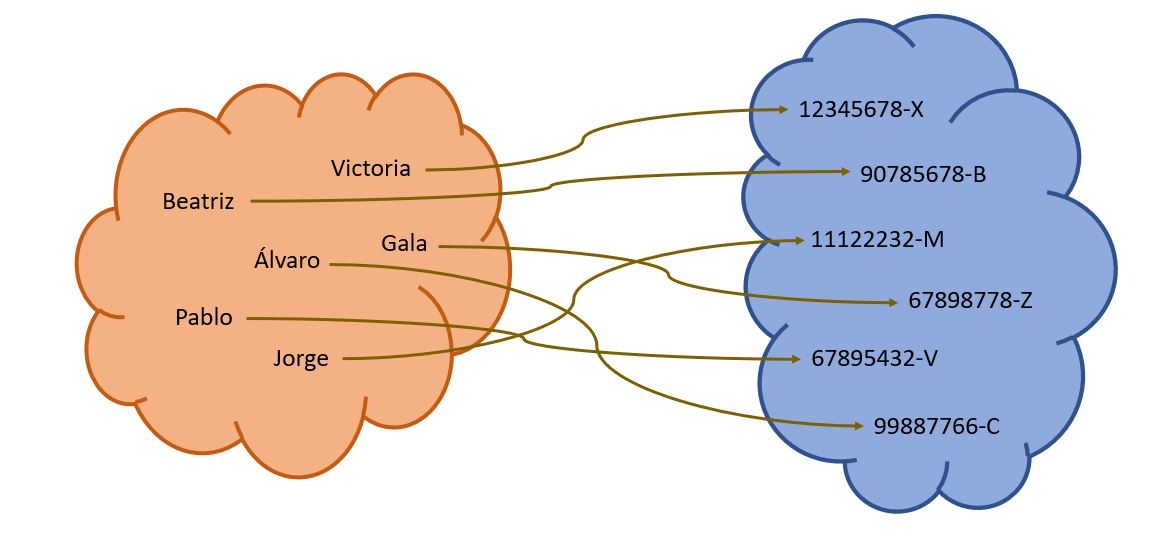
\includegraphics{samples/imagenes/imagenConcepto.jpg}

\begin{definition}
Una \emph{función} es una correspondencia tal que a cada valor del primer conjunto le corresponde un único valor del segundo conjunto. 
\end{definition}
\geogebra{bm9zpgfh}
Un ejemplo claro de función podría ser la relación existente entre un hijo y su madre, ya que cada hijo tiene una única madre.

Existen diferentes formas de expresar una función:
\begin{itemize}
	\item \emph{Mediante un enunciado verbal.}
	\item \emph{Mediante una gráfica.}
	\item \emph{Mediante una fórmula matemática.}
	\item \emph{Mediante una fórmula matemática.}
\end{itemize}

\subsubsection{Ejercicios.}
\begin{enumerate}
	\item Introduzca en la barra de entrada las siguientes funciones, de manera similar a la indicada en el ejemplo anterior, y observa la gráfica de representación de cada una de las funciones.\\
	\begin{itemize}
		\item $f(x) = 3x+2$
		\item $g(x) = \dfrac{x^2-3}{x+5}$
		\item $h(x) = \sqrt{x+5}$
		\item $j(x) = \dfrac{2x^2+1}{3x-5}$
		\item $k(x) = \log (x^2)$
		\item $p(x) = 3\cos(3x)$
	\end{itemize}
	\geogebra[ai=true, stb=true]{tc5pbmae}
	\item Cite todas las familias de funciones a las que pertenecen cada una de las siguientes:
	\begin{itemize}
		\item $f(x) = 2x^3-3x$
		\item $f(x) = 6x+2$
		\item $f(x) = -\sqrt{x+1}$
		\item $f(x) = \tan (x-4)$
		\item $f(x) = \dfrac{2x-1}{x+7}$
		\item $f(x) = \log(x^2)$
	\end{itemize}

\end{enumerate}

\begin{ex}[sol after]
	Enunciado ejercicio.
	\lipsum[1]
	\begin{sol}
		Solución a continuación.
		\lipsum[1]
	\end{sol}
\end{ex}
